\begin{figure}[H]
	\centering
	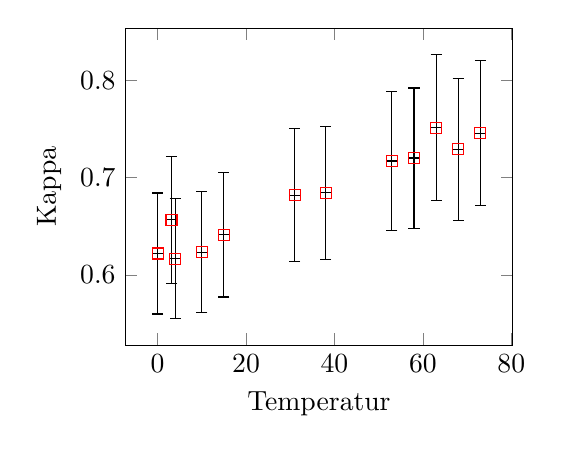
\begin{tikzpicture}
		\pgfplotsset{width=6.5cm,compat=1.3,legend style={font=\footnotesize}}
		\begin{axis}[xlabel={Temperatur},ylabel={Kappa},legend cell align=left,legend pos=north west]
		\addplot+[only marks,color=red,mark=square,error bars/.cd,x dir=both,x explicit,y dir=both,y explicit,error bar style={color=black}] table[x=X,y=Y,x error=xerror,y error=yerror,row sep=\\]{
			X	Y	xerror	yerror	\\
			3.141592653589793	0.6565661435410208	0	0.06565661435410208	\\
			73	0.745651428687384	0	0.0745651428687384	\\
			68	0.7291896973891191	0	0.07291896973891192	\\
			63	0.7514142988993405	0	0.07514142988993405	\\
			58	0.7202039843396486	0	0.07202039843396486	\\
			53	0.7171452345550323	0	0.07171452345550323	\\
			38	0.6845595922438421	0	0.06845595922438422	\\
			31	0.682063770279751	0	0.06820637702797509	\\
			15	0.6413677738717087	0	0.06413677738717087	\\
			10	0.623492704217991	0	0.0623492704217991	\\
			4	0.6165815992240085	0	0.06165815992240085	\\
			0	0.622000108043746	0	0.062200010804374595	\\
		};		% \addlegendentry{Messpunkte Datensatz 0}
		\end{axis}
		\end{tikzpicture}
	\caption{$\kappa(T)$}
	\label{fig:KappaTemperatur}
\end{figure}